\section{Induktives Laden}
Um den Energiespeicher des Dojos aufladen zu können, wird eine induktive Ladeschaltung eingebaut. In einer externen Ladevorrichtung wird die Netzspannung umgewandelt und auf eine Spule gegeben. Diese Spule erzeugt somit ein elektrisches Feld. Ist der Dojo in Reichweite zu dieser Apparatur und somit im induzierten Energiefeld, wird die Energie von diesem in elektromagnetischer Form in den Dojo transportiert und dort umgewandelt. In der Spule, die sich im Dojo befindet, wird so eine Wechselspannung induziert. Um diese Spannung für die Akkuladung nutzbar zu machen, wird diese mithilfe eines Gleichrichters angepasst und anschliessend noch geglättet. Die induktive Lademethode ermöglicht es, ein komplett geschlossenes Gehäuse zu verwenden. Dadurch ist der Dojo vor eindringender Feuchtigkeit oder Schmutz geschützt. Des Weiteren ist so seine Lebenszeit verlängert. Aufgrund fehlender Anschlüsse können auch keine Abnutzungserscheinungen auftreten, welche durch häufiges ein- und ausstecken auftreten können. 

\begin{figure}[H]
\begin{center}
	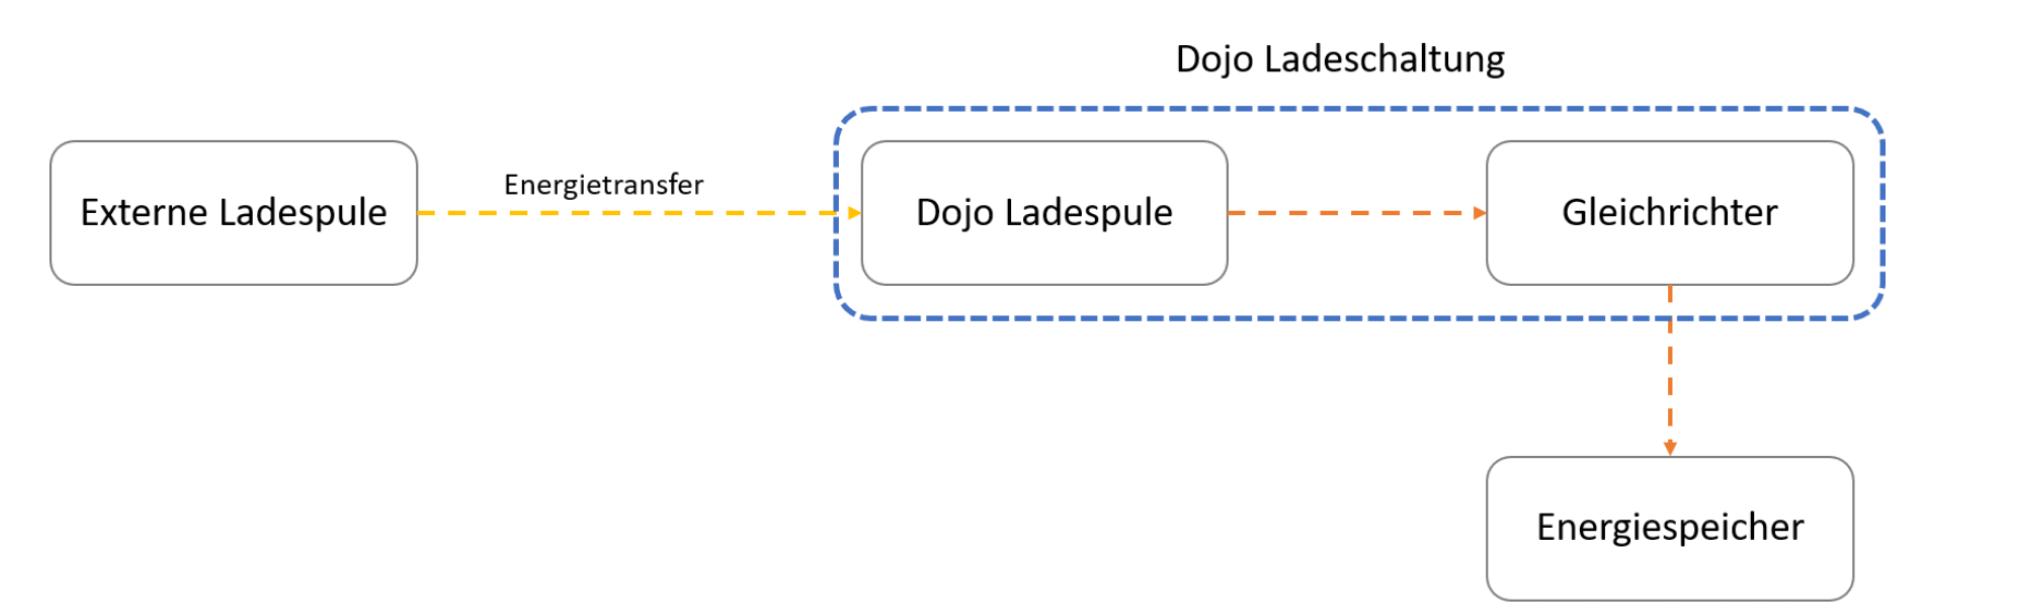
\includegraphics[width=160mm]{data/Induktion.png}
	\caption{Grobstruktur der Bluetooth-Software} %picture caption
	\label{fig:first_layer}
\end{center}
\end{figure}